\documentclass[hidelinks, a4paper]{report}
\usepackage[english]{babel}
\usepackage[utf8]{inputenc}
\usepackage[T1]{fontenc}

%%Comments
%Use \myquote{word} for correct quotation marks on word.

%%Packages
\usepackage{hyperref}
\usepackage{graphicx}
\usepackage{pdfpages}
\usepackage{supertabular}
\usepackage{float}
\usepackage{todonotes}

%%Commands
%Pretty tables
\renewcommand{\arraystretch}{1.5}
%Easy correct quotation
\newcommand{\myquote}[1]{``{#1}''}
%prettier chapters
\usepackage{titlesec, blindtext, color}
\definecolor{gray75}{gray}{0.75}
\newcommand{\hsp}{\hspace{20pt}}
\titleformat{\chapter}[hang]{\Huge\bfseries}{\thechapter\hsp\textcolor{gray75}{|}\hsp}{0pt}{\Huge\bfseries}


%%Document start
\begin{document}

\title{An Examination of the Recruitment Process at Valcon}
\author{Jakob Ambeck Vase \and Jonas Kastberg Hinrichsen \and Jakob Merrild \and Mikkel Frikke Madsen \and Martin Juul Petersen}
\listoftodos[Todos]

%%Preface
\maketitle
\tableofcontents
%\listoffigures
%%Content
\chapter{Introduction}
\todo{Should we have chapter numbers?}
\section{Problem introduction}
This report is written as part of an analysis of a problem at Valcon Group.
The problem analysed is as follows:

\emph{How can the Valcon Group save time and reduce frustration in the IT department by improving the process of new employee registration?}
\\
A more detailed version of the problem statement can be found in appendix \ref{app:problem_statement}.

The problem has been formulated based on an initial meeting with Danni Jensen, who stated that the process should \myquote{identificeres, automatiseres og effektiviseres}.(Appendix \ref{app:danni_initiation})
During the same meeting Danni stated that the most important success criteria for him was that the report could be used to document the existence of the problem.

\section{Methods}
In order to fully understand and analyse the problem we have interviewed several employees of the Valcon Group.
Additionally we have conducted some minor observations of the work processes in the Accounting and IT departments.
We would have liked to supplement this with a questionnaire given to all employees at Valcon Group.
The purpose of the questionnaire would be to get an understanding of the employees perspectives on the process of new employee registration.
However, it was deemed that such a questionnaire would take up too much valuable time from the employees.
\todo{Merge methods section with approach.tex}
\section{List of activities}
Based on the process analysis in which we identified the work areas relevant to the process, we conducted various interviews.
We chose to begin with interviewing Lisbeth (of accounting) and Peter (of IT), as they are the ones most affected by the process.
We chose to interview Hanne (NBA) as well, as she is the initiator of the process at Valcon.
Finally, we chose to observe both IT and accounting, to get a sense of the work flow there.

When we analyzed the data, we realized that we had to interview Jytte (process initiator at OMT) as well, as much of the problem originates in OMT.
\todo{Why no quantitative analysis? SOURCE}
\todo{Why no Valcon/OMT recruiter interview? SOURCE}

\section{Solutions Already Underway}
During our initial meeting with Valcon, we were informed that they were already aware that their current HR system did not perform satisfactory, and that they were looking at new systems to replace the old. We kept this in mind as we conducted interviews and investigated possible solutions, as it was a key factor in improving the process.

\section{Notes}
During the analysis we realized that OMT was an integral part of the problem, and started to analyze them as well.
Our scope got too big, so we limited the amount of gathered knowledge from OMT to a single interview with a recruiter at OMT with a key person in regards to the process. 

We realize that this limits our general understanding of the procress, and thus most of the solutions proposed in regards to OMT are conducted based on limited knowledge, and should be further revised before implemented. 

\chapter{In-line analysis \\ Understanding Valcon's goals}
The following chapter describes our understanding of Valcon as a company. This includes the environment in which they operate, an analysis of their business model, their business and IT strategies, and an identification of which work domains that affect the problem.

We conducted the analysis before realising that OMT was a big part of the problem, and therefore the analysis in regards to OMT is very limited.

\section{Business environment}
As we are working with internal support functions, we provide only summaries of our environment analyses here.
\subsection{Valcon's environment}
Valcon operates within an competitive environment where image and contacts are key. 
There's a great need for experienced and knowledgeable consultants but there's also a lot of competition in the field.
Not because there are a lot of competitors within the fields that Valcon works in, but rather because the competitors are the same every time.
This means they know each other and know exactly what kind of prices and quality the opposing firms will bring.
Due to this, Valcon's business strategy has been to hire the best and brightest employees and accept the fact that they're unable to be the cheapest organisation to hire.

They sell themselves mainly on knowledge and quality, rather than on price and pride themselves on being a company capable of the entire consultation process, from analysis to implementation.

They refer to themselves as the 'how' company, as they are often employed in projects where a competing consultation firm has been hired to write the analysis report and figure out 'what' to do. 
Valcon are then employed to conclude the project by implementing the solution.

Valcon's biggest threat is losing their consultants.
Consultants are drawn towards new and exciting opportunities, while working for the same company for a long time gets increasingly stale.
This means that sooner or later a consultant will grow tired of the current challenges he's facing and move on to another company. \todo{SOURCES}
\subsection{OMT's environment}
OMT primarily works with warships, a field they're not facing a lot of competition within. 
This also enables them to subcontract other companies, since they're not direct competition and therefore don't mind.
A more thorough investigation of OMT's environment can be found in appendix \ref{app:OMT_environment}.
\section{Valcon's business model}
The business canvas gives an overview of Valcon's business.
Based on our analysis we have the following understanding of Valcon's canvas.
\begin{figure}[!htp]
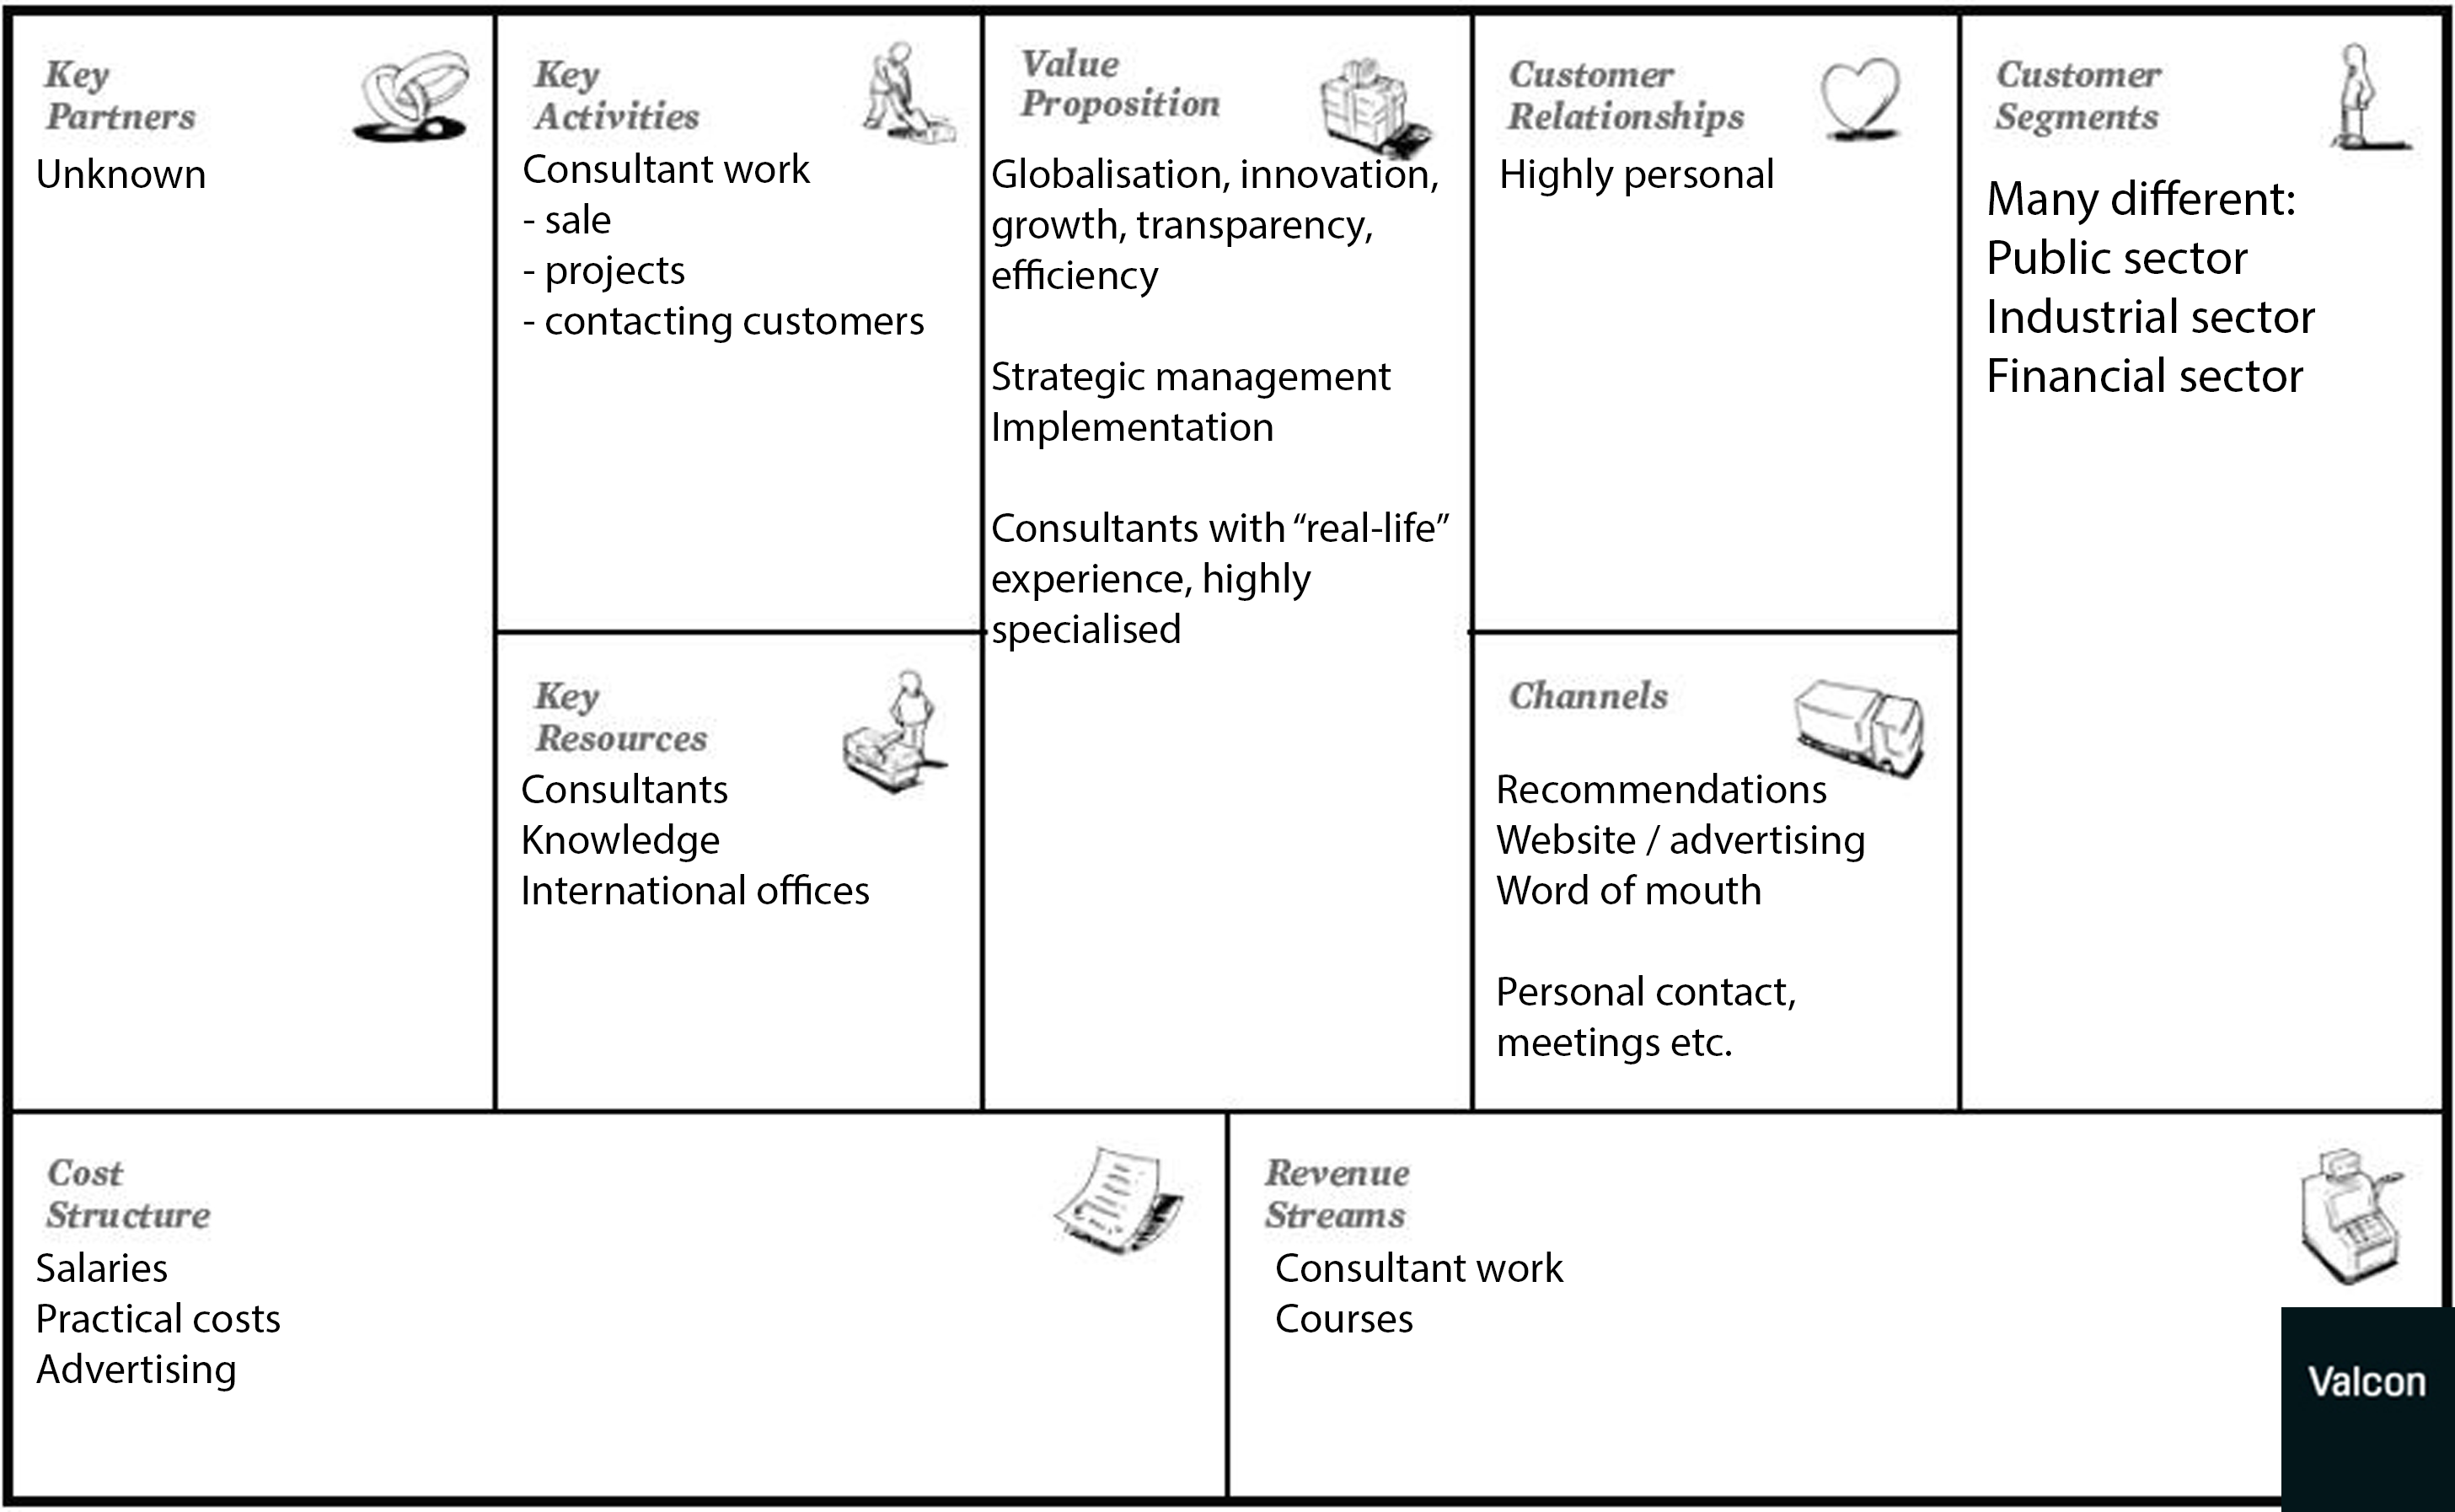
\includegraphics[width=\textwidth]{inline/business-model-canvas.png}
\caption{Valcon's business canvas.}
\label{fig:canvas}
\end{figure}

In relation to the problem it is important to note that the consultants are key resources for Valcon's business
as they are the ones who generate revenue.
As such it is important that they are able to perform their work effectively as soon as they start working at Valcon.
\section{Business strategy, IT strategy and company values}
\subsubsection{Business strategy}
We were not able to acquire Valcon's business strategy, as it is not public and Valcon were not interested in sharing it. (Source: Danni: "Det er korrekt at Valcon gruppens konkrete business strategi ikke er tilgængelig" (appendix \ref{app:business_strategy_refusal})). 
However, we were able to glean some of it through the interviews and meetings:

Valcon is in rapid growth and have a continued focus on keeping this growth as high as possible. 

(Sources: appendix \quoteref{app:danni_initiation}{danni_init_eksplosiv_vekst} and appendix \quoteref{app:danni_initiation}{danni_init_business_strategy_vekst}).

\subsubsection{IT strategy}
Valcon's IT strategy focuses on streamlining IT activities, being cost efficient, outsourcing labor intensive tasks, making work easier for the consultants, few but strong partnerships and choosing off-the-shelf systems instead of customized systems.

See appendix \ref{app:it_strategy} for the original document.

\subsubsection{Company values}
Valcon is guided by four values internally: Integrity, joy, performance, and competence.
Furthermore they value a flat hierarchy.
(Source: appendix \quoteref{app:danni_initiation}{danni_init_firmastruktur}).
\section{Work domains}
Entering newly hired employees into the systems at Valcon and requisitioning the required hardware is currently a stressful process.

Initiators of the process in both Valcon and OMT send information to accounting, who proceeds to enter information into some systems while IT enters information into other systems, sets the hardware for the new employee up, and sends it to him/her.
The new employee is contacted both by the initiators and IT, and sometimes by accounting as well.

But the core of the problem is that the process sometimes has to be very quick.
In that case, the initiators initiate the process both in IT and accounting at the same time, leading to more stress and intercommunication between them.

Looking at the process it seems essential to take a deeper look at the following work areas in order to get a better understanding of the problem:
\begin{itemize}
\item Recruitment (the initiators)
\item Accounting
\item IT
\end{itemize}

A visual representation of the organization as well as the work domains to research can be seen in appendix \ref{app:OrganizationalChart}
\section{Conclusion}
This section aims to explain how the recruitment process problem, we are dealing with, is relevant to Valcon as a whole.\\

\noindent Part of Valcon's business strategy is to keep a high growth rate for the company.
A high growth rate means many new employees.
All employments go through Group Support Functions (IT and accounting) in the recruitment process.
Group Support Functions has problems dealing with the current amount of employments.

Since Valcon intends to keep growing and Group Support Functions have problems keeping up, there is a need to optimize the process.
\chapter{In-depth analysis \\ Understanding the problem}
The following chapter will explain our approach to analyzing the process, describe the process in some detail and highlight key findings.

\section{Process analysis approach}
Based on the process analysis in which we identified the work areas relevant to the process, we conducted various interviews.
We chose to begin with interviewing Lisbeth (of accounting) and Peter (of IT), as they are the ones most affected by the process.
We chose to interview Hanne (NBA) as well, as she is the initiator of the process at Valcon.
Finally, we chose to observe both IT and accounting, to get a sense of the work flow there.

When we analyzed the data, we realized that we had to interview Jytte (process initiator at OMT) as well, as much of the problem originates in OMT.
\todo{Why no quantitative analysis? SOURCE}
\todo{Why no Valcon/OMT recruiter interview? SOURCE}
\section{Process description}
The process starts when a new employee has been hired.
An initiator (often Hanne or Jytte, sometimes other people) contacts accounting with information on the new employee.
A contract has to be formulated and, if there is information missing, the new employee has to be contacted in order to complete their particulars.

The information is entered into QHR and IT is contacted to let them know that a new employee has been hired.
IT then uses the information in QHR to create a new user in AD and give them a mailbox on the Exchange Server, and contacts accounting again with the employee's initials.
Accounting, after receiving the initials, enters the employee's particulars in Maconomy and Bluegarden (or in the case of foreign departments, the relevant salary system for that country).

At the same time IT contacts the new employee about their preferences for phone and internet.
When they have received these from the employee they contact Valcon's communications provider in order to set the new employee up according to their preferences.

Also at the same time, a PC is set up by IT according to the new employee's needs, based on which department they will work for.
Finally information about the handed out gear is recorded in TechAdm.

A visual representation of the process can be found in appendix \ref{app:ProcessChart}
\section{Key findings}
\subsection{Results from interviews}
There are several reasons why the current recruitment process needs to be optimized.

1. The main frustrations in the IT-department are that some recruitments occur with very short notice, and that data occasionally is incomplete.
(Appendix \completeref{app:peter} lines \lineref{peter_datamangel}, \lineref{peter_frustration1}, \lineref{peter_frustration2}, and \lineref{peter_frustration3})
The short notices are mainly rooted in recruitment of subcontractors in OMT, while the incomplete data occurs both with recruitments in Valcon and OMT.
(Appendix \quoteref{app:peter}{peter_short_notice})
Part of the problem with incomplete data is that the recruiters are not aware of exactly what information is needed in order to set a new employee up correctly.
(Appendix \quoteref{app:jytte}{jytte_stamdata})

We think that some of the frustration stems from IT not having a standard process for when data is incomplete.

2. The main frustration in Accounting is that employee data is managed in many different systems and needs to be copied manually.
(Appendix \quoteref{app:lisbeth}{lisbeth_manuelle_indtastninger})
Each employee in the recruitment process maintains their data on the new employees in individual spreadsheets.
(Appendix \quoteref{app:lisbeth}{lisbeth_ark})
This is problematic, as non-standard processes are hard to pass on.

3. A lot of time is spent communicating information back and forth between Accounting and Recruitment.
(Appendix \quoteref{app:lisbeth}{lisbeth_vende_tilbage})
Similarly time is spent communicating the information to the IT-department.
(Appendix \quoteref{app:lisbeth}{lisbeth_IT})
Accounting and IT want communication to be more standardized, while Recruitment finds it problematic because all data isn't necessarily available by the time of recruitment.
(Appendix \quoteref{app:lisbeth}{lisbeth_standardiseret_proces}, \quoteref{app:peter}{peter_standardiseret_proces} and \quoteref{app:hanne_interview}{hanne_ikke_standardiseret_proces})
Forcing standardized communication might put additional pressure on the consultant/manager in charge of the recruitment, which should be avoided.
(Source: appendix \quoteref{app:hanne_interview}{hanne_standardised})
At OMT, requiring standardized communication might be possible.
(Source: appendix \quoteref{app:jytte}{jytte_standardised})

With a common system for keeping the information, 2. and 3. could be avoided, as everyone could view the data within that system.

4. Time is spent on routine tasks, such as defining new initials.
(Appendix \quoteref{app:peter}{peter_initialer})
This could possibly be automated.

5. Time is wasted waiting for other employees, as IT doesn't have standard processes for communication.
(Appendix \quoteref{app:emails}{matias_on_structure})
This is outside our scope, but should be investigated.

A visual representation of the chain of problems can be found in appendix \ref{app:ProblemChain}.
A transcript of the interviews can be found in appendix \ref{app:interviews}.

\subsection{The numbers}
\begin{wrapfigure}{r}{0.5\textwidth}
\vspace{-20pt}
\centering
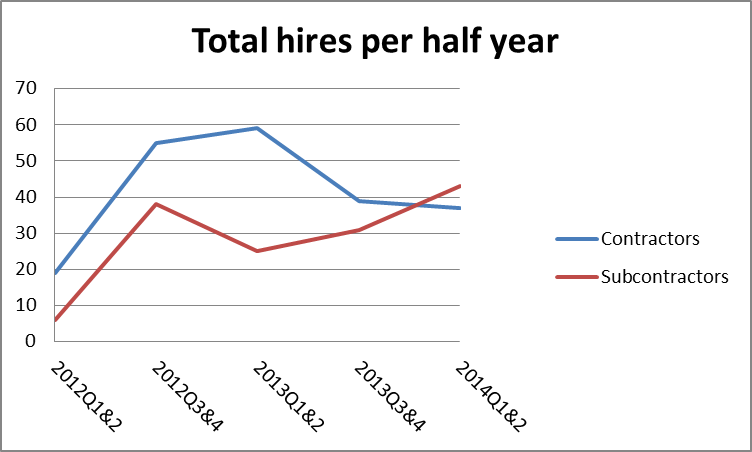
\includegraphics[width=0.45\textwidth]{appendix/total_hires_per_half_year.png}
\label{fig:total_hires_per_half_year}
%\caption{Total number of new hires per half year.}
\end{wrapfigure}
Looking at the number of new hires in Valcon we got an impression of the scope of the problem.
Even though there are some fluctuations there is a trend toward a growth in the number of hires.
This corresponds with the expressed business strategy of growth.
However, the data is not entirely conclusive, as we have only been able to look at the number of new hires within the last 30 months.
A table with all the numbers of new hires can be found in appendix \ref{app:recruitment_data} together with additional graphs.
\chapter{Innovation \\ Possible solutions}
In this section we will describe the most relevant solution propositions and, on the basis of a cost-benefit analysis, document the impact on the company as a whole.

\section{Solutions}
Please refer to appendix \ref{app:solution_propositions} (p. \pageref{app:solution_propositions}) for a complete list of solution propositions. Each solutions is listed with a verdict of its suitability, sorting out the most improbable.
The most relevant solutions are subject to cost/benefit analysis in the following sections. \todo{Implementation i hvert afsnit.}
\todo{Why no 1 solution but many?}

\subsection{Template for recruitment}
\emph{Description:} Create a template for recruitment so recruiters know what information is required. A template also functions as a checklist, ensuring that the writer knows what information to send.

\emph{Pros:} Could reduce the amount of missing information in the initial email to accounting or IT. 
Also leads to a better defined process.

\emph{Cons:} Requires additional work by recruiter. 
If template is too information heavy, some may ignore it.
Valcon employees dislike forms and rigid processes, so they may ignore it.

\subsubsection{Finance}

\subsubsection{Conclusion} Creating a template for OMT recruitment seems a good idea.
Creating one for Valcon would be a bad idea, as it would take time from management and consultants, but creating one for Hanne might work, as she would be reminded of the information required.

\subsection{Change of attitude toward IT}
\emph{Description:} Change the company attitude toward IT, from the current "they are there to fix my problems" to "they are there if I really need them".
We do not know how to implement this, but as Valcon is a consulting company, we assume they have a strategy for this case.

\emph{Pros:} May reduce the number of edge cases, recruiters would be more likely to send recruitment information in early or give warning that a quick recruitment is coming up.
Doesn't require extra time from recruiters.

\emph{Cons:} It would be hard to measure the success of the change - when is an attitude changed? - but measuring the result of the change could be done.

\subsubsection{Finance} For benefit, measure current number of edge cases and their average time cost.
Make a guess as to how many of these would be avoided with the change (15\%?).
Compute hours gained and multiply with wages for IT.
As for cost, 8-10 hours of work for a consultant might be enough to implement this.

\subsubsection{Conclusion} 

\subsection{Buffer of computers}
\emph{Description:} Keep 2-3 pre-installed computers ready for use at OMT and at Valcon, for emergencies or very quick recruitments.

\emph{Pros:} Would reduce response times to urgent recruitments.
Also useful if an employee's computer breaks, to reduce downtime.

\emph{Cons:} Needs a little more managing from IT, as
computers will need to be kept updated and ready.
As all computers are not in use, this creates a small overhead.

\subsubsection{Finance} Free. Benefit in time gained. Resources lying dormant.

\subsubsection{Conclusion}

\subsection{New HR system}
\emph{Description:} Acquire a new HR system to facilitate communication between accounting, IT, and recruiters.
Valcon is already looking at HR systems.

\emph{Pros:} Recruitment process becomes more standardized, as it always follows the same path.
Information becomes more consistent, as personal spreadsheets are less needed. 
This also safeguards against employees leaving.
Errors are less likely, as number of manual entries of information is reduced.

\emph{Cons:} Costly to implement, requires training of accounting, IT, and recruiter employees.
Also requires maintenance.

\subsubsection{Finance} +: Try to put a price on errors, count how many of them occur, guess how many will be eliminated, sum their costs.
Price of current HR system (Lotus Notes).

-: Price of new HR system.
Price of data transfer.
Price of training.
Price of maintenance.

\subsubsection{Conclusion} This solution is very necessary, as it is the only way information becomes more consistent.

\subsection{Other small improvements}

Write! \todo{The small improvements need including in the report.}

\section{Other recommendations}
Need rewriting \todo{Is this section good? Is it relevant?}

\subsection{Analyze OMT process}
Conduct an analysis of whether the OMT process can be improved so they know further in advance who and when someone is needed, so the number of urgent cases can be reduced.

\subsection{Further automation of install process}
The install process is very time consuming, and is a candidate for automation.
Looking into whether more of it could be automated could save time.


\appendix
\chapter{Project Agreement}
\section{Premise}

\subsection{Background}
In Valcon, the process of registering new employees is characterized by loose organization. This is a problem, as the company is growing quickly and many employees are recruited, and specialists are recruited for short periods of time. We have been asked to research this process and explore possible solutions, and finally to write a business case explaining the benefits and drawbacks of different solutions.

\subsection{Assignment and Objective}
The objective of the project is to research the process of registering new employees. HR departments in both OMT and Valcon collect information on the new employee and send this to either an accountant or the IT department, depending on what they need done first. This creates an unnecessary need for communication between the IT department and the accountant, which might be avoided if the process was standardized. The accountant enters financial and personal information into a system (QHR), which the IT department then uses to send a computer, setup internet connection and phone accounts, and enter the employee into the central system (AD). To further understand the current situation, the project group will conduct an ethnographic analysis of the process, in an attempt to discover parts of the process that could be effectivised, and look at ways to do so.

\subsection{Financial framework}
There will be no money involved in the project.
The resulting report of the project may be used freely by Valcon.

\subsection{Critical factors}
\textbf{Success factors:}
The solutions proposed should reduce the time, complexity and effort it takes to enter a new employee into the system.
The Business Case provided by the group must, regardless of the solutions proposed, be useable as documentation for the existence of the problem.
The solution proposed must still make use of the Active Directory which Valcon uses for managing their IT structure.
\textbf{Critical preconditions:}
We need to be able to get the time needed from the resources mentioned below.

\section{Organization}
\subsection{Project organization}
The project organization consists of two groups. The project group at ITU consists of Michael Frikke Madsen, Jonas Kastberg Hinrichsen, Martin Juul Petersen, Jakob Ambeck Vase, and Jakob Merrild. They report to Danni Jensen at Valcon.

\subsection{Resources}
The time of the project group.
3 meetings (with a 4th optional one) with Danni Jensen of appr. 1 hour each.
One or two interviews with each key employee in the process (Lisbeth, Peter, Mathias, HR) of appr. 30 min. each.
Open doors, for observing the work practises involved in the process.

\subsection{Stakeholders}
Danni Jensen
Lisbeth Justesen
The IT department of Valcon
HR departments of OMT and Valcon

\subsection{Agreements}
The following agreements were made:
The project group can conduct observations of public areas at Valcon without prior notice.
In order to conduct interviews with and observations of individuals, an agreement must be made with Danni Jensen, who must authorize the project group to initiate contact with the person to be interviewed. 
After the initial contact has been made, the project group is free to contact the person directly in order to make an appointment.

\section{Method}
\subsection{Overall Approach}
The overall approach to the project will be using the MUST method. The MUST method consists of the following four phases:
Initiation phase, where we agree on the problem and a contract
In-Line analysis, where the project group will align the project’s goals with the company’s IT and business strategy
In-depth analysis, where the project group will observe and document the relevant work practices
Innovation phase, where solutions will be investigated and optionally presented

\subsection{Plan}
\begin{itemize}
\item[13/10] - End of In-Line phase.
\item[15/10] - Meeting after In-Line and before In-Depth phases.
\item[10/11] - End of In-Depth phase.
\item[14/11] - Meeting after In-Depth and before Innovation phases.
\item[4/12] - End of Innovation phase
\item[Before] 17/12 - Delivery of Business Case
\item[??] - Optional meeting after Innovation phase.
\end{itemize}

\subsection{Signatures}

\end{document}